\chapter{Experimentación}\label{chapter:implementation}

En el capítulo se describe los conjuntos de datos utilizados para el entrenamiento y validación del modelo 
propuesto. Se mencionan las herramientas utilizadas para la confección del software. Además se describe el 
proceso de experimentación y evaluación de los modelos construídos con los conjuntos de datos. Finalmente
se presentan los resultados obtenidos con los modelos al aplicarles las cartas a la dirección extraídas 
del periódico Granma. 

\section{Conjuntos de Datos}

TODO PONER COMO SE REALIZO LA CONFECCION DEL CONJUNTO DE DATOS EN LOS MODELOS

Para el entrenamiento de los modelos propuestos se utilizaron corpus diferentes, estos
presentas esquemas de anotación distintos entre sí. Dado que todos los corpus estaban en inglés, 
se les aplicó previamente el algoritmo de proyección de corpus propuesto y se crearon sus respectivas
versiones en español. A los conjuntos de entrenamientos se le aplicó la técnica de \emph{backtranslation}
para aumentar su tamaño. Como conjunto para validar los modelos fueron usadas las cartas a la dirección
extraídas del periódico Granma.

\subsection{Procesamiento de los datos}

Los conjuntos de datos a analizar se les realizó un aumento de datos mediante le técnica de \emph{backtranslation}.
Esto contribuyó a duplicar la cantidad de elementos disponibles. Los resultados obtenidos al compara los 
elementos originales con los aumentados se reflejan en la tabla (Tabla \ref{table:data_augmentation}).

\begin{table}[h!]
	\begin{center}
		\begin{tabular}{|c|c|c|c|c|} \hline
		Corpus		            &  Jaccard	& Levenshtein	& Palabras originales / aumentadas   \\ \hline
        Ensayos Argumentativos	&  0.69		                & 96		                    & 1.00	  \\ \hline
		CDCP                    &  0.72	                    & 30		                    & 1.02	  \\ \hline
        AbsTRCT                 &  0.74		                & 86		                    & 1.04	  \\ \hline
		\end{tabular}
	\caption{Datos promedios comparando los textos originales con los aumentados.}\label{table:data_augmentation}
	\end{center}
\end{table}

Los datos extraídos muestran que se logró una variación pequeña en los datos, consiguiendo variaciones en palabras aunque conservando la 
longitud original del texto.

Todos los conjuntos de datos están originalmente en inglés, por lo tanto se les aplicó el algoritmo de proyección
de corpus para obtener un corpus en español para ser usado en el entrenamiento de los modelos. 
Para la traducción automática se utilizó los servicios de Google Translator [\cite{translateGoogle}]. Para calcular las 
alineaciones de palabras se probaron dos algoritmos, FastAlign [\cite{dyer2013fastalign}] y AwesomeAlign 
[\cite{dou2021word}]. Se observó que el primero, aunque es más rápido posee una calidad menor en los resultados,
el segundo posee una mayor calidad aunque requiere de mayor tiempo y recursos para ejecutarse. Para los experimentos
se usó finalmente AwesomeAlign. La proyección de las etiquetas fue llevada a cabo por el algoritmo propuesto 
en [\cite{eger2018cross}].

\subsection{Ensayos Argumentativos}\label{corpus:persuasive_essays}

Este corpus [\cite{stab2017parsing}] presenta unos 402 documentos, dividido por los autores en 286 documentos para entrenamiento (70\%), 
80 para prueba (20\%) y 36 para validación (10\%). Los contenidos de estos son ensayos de estudiantes en los que 
se argumentan sobre temas como: cooperar o competir, contribuciones de la tecnología a la sociedad.
Las anotaciones de las UDA se conforman por segmentos de textos considerados argumentativos, estos segmentos son 
clasificados en \emph{MajorClaim} (751 12\%), \emph{Claim} (1506 25\%) y \emph{Premise} (3832 63\%).
La estructura de las relaciones entre las UDA conforman árboles en los que se tienen como raíz las 
\emph{MajorClaim} del texto. Las relaciones solo estan permitidas entre \emph{Premise-Premise} y \emph{Premise-Claim}, clasificadas
en \emph{attack} (219 6\%) y \emph{support} (3613 94\%). Las relaciones entre \emph{Claim} y \emph{MajorClaim} son anotadas de manera diferente, por medio de 
darle a las \emph{Claim} una clasificación de si está a favor (1228) o en contra (278) de las \emph{MajorClaim} del documento.
Para el análisis de este corpus se consideraron las relaciones \emph{Claim-MajorClaim} de igual manera que las otras,
al convertir estas posiciones en relacines. El número final con la inclusión de estas aumenta a 715 (10\%) de ataque y 
5958 (90\%) de apoyo.

\subsection{CDCP}\label{corpus:cdcp}

El corpus [\cite{niculae2017argument}] está conformado por 731 comentarios de usuarios extraídos de la web bajo el tema de 
prácticas de cobro de deudas a los consumidores (CDCP por sus siglas en inglés \emph{Consumer Debt Collection Practices}).
Las UDA se encuentran segmentadas en oraciones y todas se consideran argumentativas, estas son clasificadas en 
\emph{policy} (815 17\%), \emph{value} (2180 45\%), \emph{fact} (785 16\%), \emph{testimony} (1116 21\%) y \emph{reference} (32 1\%). 
Las relaciones se encuentran clasificadas en \emph{reason} (1352 97\%) y \emph{evidence} (73 3\%).

\subsection{AbsTRCT}

AbsTRCT [\cite{mayer2020transformer}] se compone de 500 documentos sobre el estudio de 4 enfermedades diferentes,
glaucoma, hipertensión, hepatitis b y diabetes. Las UDAs constituyen oraciones, aunque no todas son consideradas
argumentativas. Estas se clasifican en \emph{MajorClaim} (93 3\%), \emph{Claim} (993 30\%) y \emph{Premise} (2198 67\%).
Las relaciones esán representadas por tres categorías: \emph{support} (1763 85\%), \emph{partial-attack} (238 12\%) y
\emph{attack} (60 3\%).

\begin{table}[h!]
	\begin{center}
		\begin{tabular}{|c|c|c|c|c|} \hline
		Corpus		            & Tokens 	& Tokens argumentativos	& UDAs   & Relaciones por UDA    \\ \hline
		Ensayos Argumentativos  & 381		& 68\% 		& 35\% 	  & 1.08		\\ \hline
		CDCP		            & 127		& 99\% 		& 97\% 	  & 0.30		\\ \hline
		AbsTRCT	                & 371		& 50\% 		& 47\% 	  & 0.63		\\ \hline
		\end{tabular}
	\caption{Información de promedios de los conjuntos de datos.}\label{table:corpus_info}
	\end{center}
\end{table}

\subsection{Cartas a la dirección}

Las cartas a la dirección constituyen un segmento del periódico Granma en los cuales son publicadas
cartas enviadas por la población o empresas a dicha entidad. En general, las cartas 
presentan dudas o problemas de la población con el objetivo de obtener respuestas del organismo
asociado. Se extrajeron 2891 cartas desde el 30 de agosto del 2013 hasta el 28 de octubre del 2022. Se 
presentan aproximadamente 975000 palabras en los datos, en promedio, la cantidad de palabras por carta es de 330.
Se encontraron 874 cartas en respuesta a cartas enviadas lo que representa un 30\% del total. Se extrajeron
los comentarios asociados a las cartas, en este sentido 987 cartas no presentan comentarios y en promedio 
se realizan 2 comentarios por carta. Los textos presentan un título y un formato relativamente libre, 
aunque en las cartas de respuesta se puede observar una firma de la persona que respondió y la entidad que 
representa. Del total de cartas se seleccionaron las que fueran en respuesta a otra y también las 
cartas que fueron respondidas para tener una mayor concentración de cartas que fueran argumentativas, 
esta selección está conformada por 1702 cartas lo que representa un 59\% del total de cartas.

TODO SI HAY TIEMPO ANOTAR LAS CARTAS CON ALGUN ESQUEMA SENCILLO (Claim, Premise) (Attack, Support) y Mapear 
las clasificaciones de los otros modelos a estas para tener algun tipo de evaluacion.

\section{Implementación}

La implementación de los modelos y algoritmos de procesamiento y visualización de datos se encuentran en 
un repositorio de GitHub\footnote{\url{https://github.com/luisoibarra/argument-mining}}. Esta implementación
está concebida para que se pueda extender fácilmente para el uso con otros idiomas además del inglés y el 
español. Se basa en una arquitectura de procesamiento secuencial en el cual cada paso del proceso realiza
una tarea específica y lo más desacoplada posible de las otras. Las tareas realizadas son:

\begin{itemize}
    \item Creación del corpus en un formato estándar. Dado que los corpus vienen en diferentes formas, este paso se realiza para trabajar sobre una misma representación de este.
    \item Proyección del corpus de un lenguaje fuente a un lenguaje objetivo.
    \begin{itemize}
        \item Traducción y alineación de oraciones.
        \item Alineación de palabras.
        \item Proyección de etiquetas.
    \end{itemize}
    \item Extracción y clasificación de UDAs.
    \item Extracción y clasificación de las relaciones entre las UDAs.
    \item Visualización de los resultados.
\end{itemize}

\subsection{Herramientas}

El lenguaje empleado para la confección del software fue \textbf{Python} [\cite{python}], este presenta 
una gran variedad de herramientas 
para el trabajo con texto, visualización de datos y la creación de modelos de aprendizaje profundo.
Se utilizó \textbf{tensorflow} [\cite{tensorflow}] en su versión 2.9.2 para la construcción y entrenamiento de los modelos. 
Para el procesamiento de los textos se utilizaron \textbf{nltk} [\cite{nltk}] y \textbf{spacy} [\cite{spacy}], con estos se realizaron tareas
como la extracción de tokens y oraciones del texto, la anotación de las etiquetas POS. Se utilizaron 
ambas bibliotecas para el procesamiento debido que en dependencia de la sitaución cada una presenta diferentes
ventajas. En el caso de \textbf{nltk} esta presenta algoritmos rápidos para el procesamiento de texto que no 
requieren de muchos recursos computacionales, sin embargo, estos algoritmos no están disponibles de inmediato
para otros lenguajes como el español. \textbf{Spacy} por su parte presenta algoritmos más certeros a costo 
de mayor tiempo de procesamiento y gasto de recursos computacionales y también presenta una cantidad de lenguajes 
disponibles mucho mayor. Para la visualización, manejo de los datos y cálculo de métricas se utilizaron 
\textbf{matplotlib} [\cite{matplotlib}], \textbf{pandas} [\cite{pandas}] y \textbf{sklearn} [\cite{sklearn}]. 
Para la recolección de las cartas del periódico Granma se utilizó \textbf{scrapy} [\cite{scrapy}].

\subsection{Visualización de resultados}

Como interfaz visual para el usuario se utilizó la herramienta Brat [\cite{brat}]. Esta herramienta permite
la visualización y edición de las estructuras argumentativas. Dado que Brat es una página web, esta se puede
desplegar y permitir su uso online.

\section{Experimentación}

Para realizar la selección del modelo se utilizó el corpus de Ensayos Argumentativos. Con este se ajustaron
las arquitecturas e hiperparámetros de los modelos propuestos. La mejor combinación de estos fue utilizada para el entrenamiento de
los corpus restantes. Finalmente los modelos fueron utilizados para anotar las cartas a la dirección. 

\subsection{Hardware}

Gran parte del procesamiento se llevo a cabo en una computadora $i5$ con $8GB$ de RAM ampliada con $4GB$ de memoria 
\emph{swap} [\cite{swap}], aunque se requirió el uso de la plataforma \textbf{Colab} [\cite{colab}] para 
el entrenamiento de algunos modelos por falta de recursos locales.

\subsection{Segmentador de UDA}

En el entrenamiento del segmentador de UDA se hicieron variaciones en la arquitectura propuesta con respecto a la
presencia o no de las siguiente componentes:

\begin{itemize}
    \item Atributos de POS en la entrada del algoritmo.
    \item Atributos extraídos por la CNN de la palabra.
    \item Atributos features extraídos por la LSTM bidireccional de la palabra.
    \item Conexiones residuales.
    \item Capa densa final.
    \item Capas de normalizaciones.
\end{itemize}

De las posibles combinaciones se presentaron 4 candidatos:

\begin{table}[h!]
	\begin{center}
		\begin{tabular}{|c|c|c|c|c|c|c|} \hline
		Modelos 	& POS       & Char-CNN  & Char-LSTM & Res       & Norm      & Densa  \\ \hline
		Modelo1		& $\times$	& $\times$    & $\times$    & $\times$	& $\times$    & $\times$ \\ \hline
		Modelo2		& $\times$	& $\checkmark$    & $\checkmark$    & $\checkmark$	& $\checkmark$    & $\times$ \\ \hline
		Modelo3		& $\checkmark$	& $\checkmark$    & $\checkmark$    & $\checkmark$	& $\checkmark$    & $\times$ \\ \hline
		Modelo4		& $\checkmark$	& $\checkmark$    & $\checkmark$    & $\checkmark$	& $\checkmark$    & $\checkmark$ \\ \hline
		\end{tabular}
	\caption{Variantes de arquitectura de los modelos de segmentación de UDA.}\label{table:segmenter_architecture_table}
	\end{center}
\end{table}

En la figura (\ref{fig:segmenter_model_loss}) se observan las diferentes curvas de aprendizaje de los modelos 
probados. Se muestra la rápida convergencia de los modelos con conexiones residuales y normalizaciones.
Se muestra también la tendencia al sobreajuste en el entrenamiento entre los pasos 17-20, en donde se detiene el 
entrenamiento para evitar el crecimiento del error de generalización.

\begin{figure}[h!]
	\begin{center}
		\begin{center}
			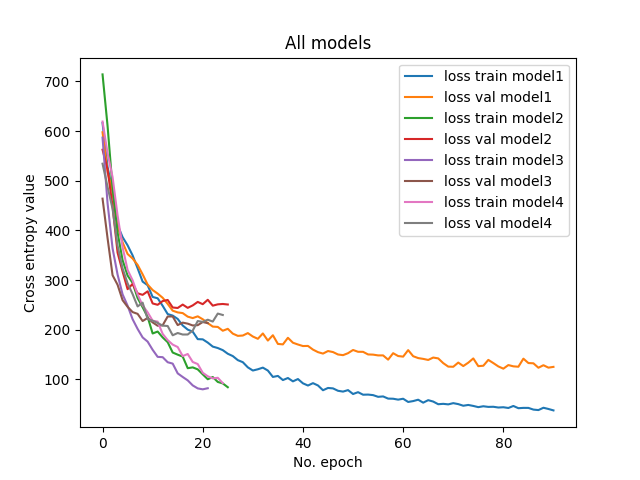
\includegraphics[scale=.9]{Graphics/persuasive_essays_all_linked_crf_loss.png}
        \end{center}
	    \caption{Pérdida de los modelos segmentadores.}\label{fig:segmenter_model_loss}
	\end{center}
\end{figure}

Las métricas \%F1 muestran que los modelos 1 y 2 presentan un desempeño menor que los 3 y 4. 
Se muestra un ligero aumento de 1\% en las 50\%F1 en el modelo 4 con respecto 
al modelo 3, aunque las métricas de F1 en el 3 superan a las de 4. Se considera que la 
segmentación como tarea principal, por lo que se selecciona como mejor modelo al 4 (\ref{fig:test_segmenter_model_metrics}).

\begin{figure}[h!]
	\begin{center}
		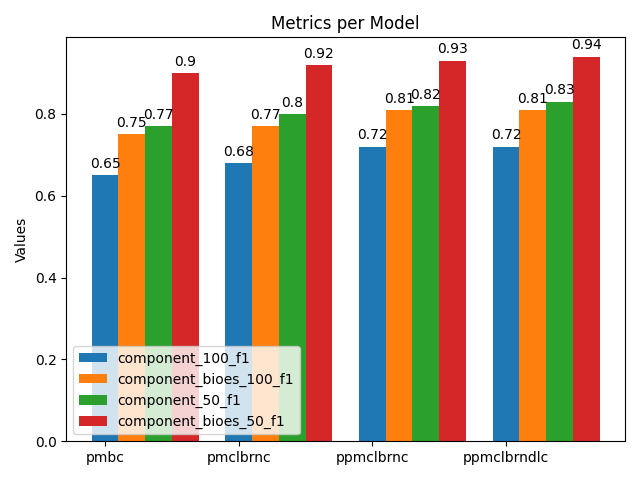
\includegraphics[scale=.4]{Graphics/persuasive_essays_all_linked_components.png}
		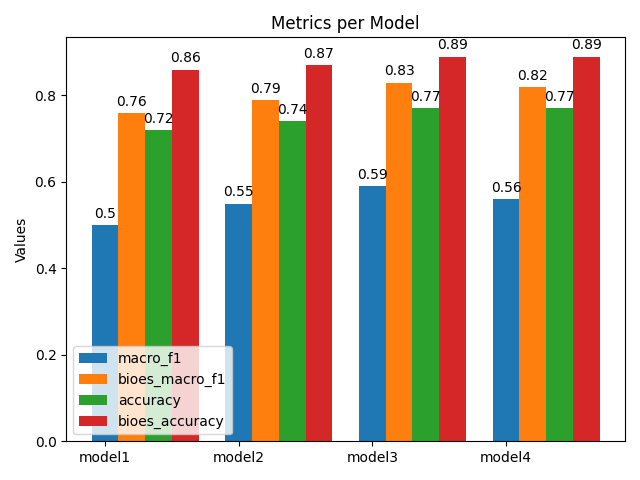
\includegraphics[scale=.4]{Graphics/persuasive_essays_all_linked_macro_micro_metrics.png}
	    \caption{Métricas del conjunto de pruebas de los modelos segmentadores.}\label{fig:test_segmenter_model_metrics}
	\end{center}
\end{figure}

El modelo seleccionado fue usado en el entrenamiento de los demás conjuntos de datos obteniendo los resultados

\begin{table}[h!]
	\begin{center}
		\begin{tabular}{|c|c|c|c|c|c|} \hline
        Corpus		            & F1 Ponderado  & Macro F1	& \emph{Accuracy} & 100\%F1 & 50\%F1  \\ \hline
        Ensayos Argumentativos  & .76           & .56 		& .77		      & .72	    & .83	       \\ \hline
        CDCP		            & .65           & .45 		& .66		      & .61	    & .68	       \\ \hline
        AbsTRCT	                & .86           & .50 		& .87		      & .61	    & .75	       \\ \hline
        \end{tabular}
	\caption{Métricas de las pruebas del segmentador de UDA.}\label{table:test_metrics_segmenter}
	\end{center}
\end{table}
\begin{table}[h!]
	\begin{center}
		\begin{tabular}{|c|c|c|c|c|c|} \hline
        Corpus		            & F1 Ponderado  & Macro F1 & \emph{accuracy} & 100\%F1 &  50\%F1   \\ \hline
        Ensayos Argumentativos  & .89           & .82	   & .89             & .81	   & .94 	   \\ \hline
        CDCP		            & .95           & .56	   & .96	         & .82	   & .93 	   \\ \hline
        AbsTRCT	                & .90           & .79	   & .91	         & .66	   & .82 	   \\ \hline
        \end{tabular}
	\caption{Métricas BIOES de las pruebas del segmentador de UDA.}\label{table:test_bioes_metrics_segmenter}
	\end{center}
\end{table}

El modelo fue aplicado a las cartas extraídas, TODO la validacion de los modelos con las cartas. ANOTAR CARTAS.

TODO Mostrar ejemplos buenos y malos
TODO Decir opiniones de los errores
TODO Hacer analisis curvas de aprendizaje -> overfitting, underfitting, representación de los datos en los conjuntos de validacion/entrenamiento

\subsection{Predictor de Enlaces}

Se entrenaron diferentes variantes de arquitecturas y hiperparámetros. Al igual que en el segmentador de
UDAs se realizó la selección del modelo que mejor se desempeñó en el conjunto de datos de Ensayos Argumentativos.
De las variaciones surgieron las siguientes propuestas:

\begin{table}[h!]
	\begin{center}
		\begin{tabular}{|c|c|c|c|c|c|c|} \hline
		Modelos  & Atención      & Pooling  & \emph{Dropout}   & Tasa de aprendizaje & Paciencia & Devolver mejores     \\ \hline
		Modelo1	 & $\times$	     & 10       & .1               & .003                & 5	      & $\times$            \\ \hline
		Modelo2	 & $\checkmark$	 &  1       & .1               & .003                & 5	      & $\times$            \\ \hline
		Modelo3	 & $\times$	     &  1       & .5               & .0015               & 5	      & $\times$            \\ \hline
		Modelo4	 & $\checkmark$	 &  1       & .5               & .0015               & 10	      & $\checkmark$        \\ \hline
		\end{tabular}
	\caption{Variantes de arquitectura de los modelos de predicción de enlaces.}\label{table:link_predictor_architecture_table}
	\end{center}
\end{table}

Las curvas de aprendizaje (Fig. \ref{fig:link_prediction_model_loss}) de los modelos muestran un nivel de sobreajuste 
elevado cuando el \emph{dropout} es pequeño. Adem'as se observan valores de p'erdida elevados lo que significa 
que el modelo le cuesta ajustarse de manera satisfactoria a los datos.

\begin{figure}[h!]
	\begin{center}
		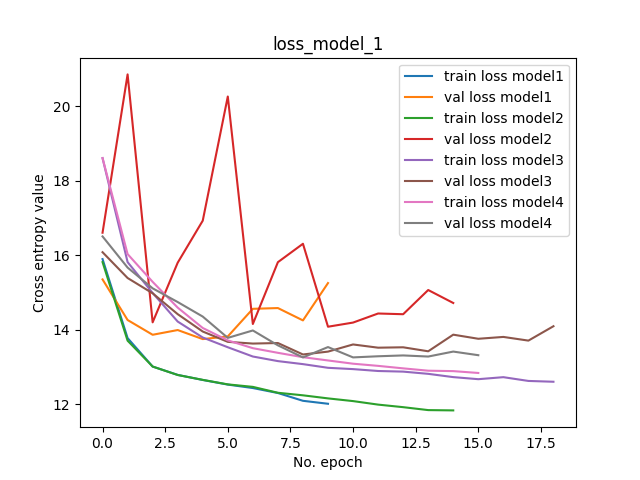
\includegraphics[scale=.9]{Graphics/persuassive_essays_all_linked_link_prediction_loss_model_1.png}
	    \caption{Curvas de aprendizaje de los modelos de predicción de enlaces.}\label{fig:link_prediction_model_loss}
	\end{center}
\end{figure}

Las m'etricas obtenidas por las diferentes versiones de los modelos muestran que TODO

\begin{figure}[h!]
	\begin{center}
		TODO M'etricas de los modelos de link prediction de persuasive essays. F1
		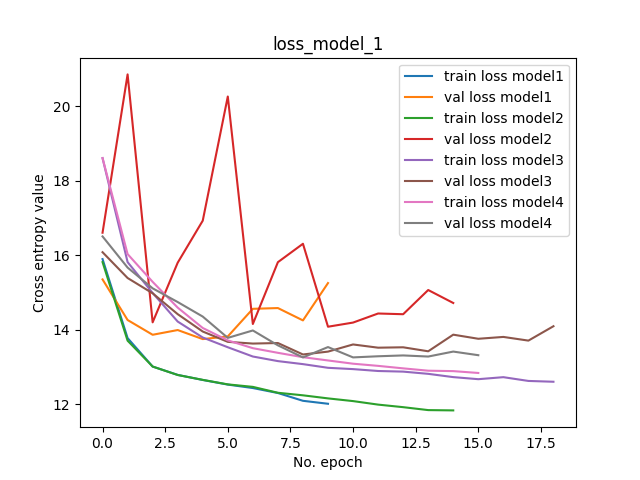
\includegraphics[scale=.9]{Graphics/persuassive_essays_all_linked_link_prediction_loss_model_1.png}
	    \caption{Curvas de aprendizaje de los modelos de predicción de enlaces.}\label{fig:link_prediction_model_loss}
	\end{center}
\end{figure}

TODO El modelo seleccionado fue X por Y

TODO FOTOS o TABLAS con los resultados relevantes en los OTROS CORPUS

\begin{table}[h!]
	\begin{center}
		\begin{tabular}{|c|c|c|c|} \hline
        Corpus		            & F1 Ponderado  & Macro F1 & \emph{Accuracy} \\ \hline
        Ensayos Argumentativos  & .89           & .82	   & .89             \\ \hline
        CDCP		            & .95           & .56	   & .96	         \\ \hline
        AbsTRCT	                & .90           & .79	   & .91	         \\ \hline
        \end{tabular}
	\caption{Métricas de predicci'on de relaciones de las pruebas del predictor de enlace.}\label{table:test_relation_metrics_link_predictor}
	\end{center}
\end{table}

\begin{table}[h!]
	\begin{center}
		\begin{tabular}{|c|c|c|c|} \hline
        Corpus		            & F1 Ponderado  & Macro F1 & \emph{Accuracy} \\ \hline
        Ensayos Argumentativos  & .89           & .82	   & .89             \\ \hline
        CDCP		            & .95           & .56	   & .96	         \\ \hline
        AbsTRCT	                & .90           & .79	   & .91	         \\ \hline
        \end{tabular}
	\caption{Métricas de predicci'on de fuente de las pruebas del predictor de enlace.}\label{table:test_source_metrics_link_predictor}
	\end{center}
\end{table}

\begin{table}[h!]
	\begin{center}
		\begin{tabular}{|c|c|c|c|} \hline
        Corpus		            & F1 Ponderado  & Macro F1 & \emph{Accuracy} \\ \hline
        Ensayos Argumentativos  & .89           & .82	   & .89             \\ \hline
        CDCP		            & .95           & .56	   & .96	         \\ \hline
        AbsTRCT	                & .90           & .79	   & .91	         \\ \hline
        \end{tabular}
	\caption{Métricas de predicci'on de objetivo de las pruebas del predictor de enlace.}\label{table:test_source_metrics_link_predictor}
	\end{center}
\end{table}

TODO Mostrar ejemplos buenos y malos
TODO Decir opiniones de los errores
TODO Hacer analisis curvas de aprendizaje -> overfitting, underfitting, representación de los datos en los conjuntos de validacion/entrenamiento

\subsection{Modelo conjunto}

Dado que la clasificación de UDAs es hecha tanto en el segmentador como en el predictor de enlaces es necesaria 
la selección de cómo se va a desambiguar esta clasificación. En base a los resultados obtenidos en el proceso
de experimentación se prefirió el resultado devuelto por el segmentador de UDAs.

TODO Poner estadisticas de ambas aproximaciones

\section{Validación}

Se entrenaron varios modelos en los diferentes corpus con los hiperparámetros seleccionados. Con estos modelos 
se procesaron las cartas y se observó cual era el que más se ajustaba a las estructuras argumentativas presentes 
en estas. Dado que la definición de UDA es algo que varía, es complejo realizar un método que evalúe de forma 
justa los resultados obtenidos por los diferentes modelos de manera conjunta. TODO PREGUNTAR COMO HACER LA VALIDACION?

\subsection{Ensayos Argumentativos}

TODO Resultados obtenidos en el Granma con el modelo.
TODO Mostrar ejemplos buenos y malos

\subsection{CDCP}

TODO Resultados obtenidos en el Granma con el modelo.
TODO Mostrar ejemplos buenos y malos

\subsection{AbsTRCT}

TODO Resultados obtenidos en el Granma con el modelo.
TODO Mostrar ejemplos buenos y malos

\subsection{Consideraciones}

TODO Poner cual modelo se considera mejor para el Granma 
TODO Decir opiniones de los errores. (El texto de Granma posee una estructura diferente al entrenante y mas libre)
